\documentclass[tikz,border=2pt]{standalone}
\usepackage{amsmath,amssymb}
\usepackage{tikz}
\usetikzlibrary{arrows.meta}

\begin{document}
% Corner point optimality: evaluating the objective at the five corners is enough; the best
% corner value, 180 at (20, 60), is the LP optimum.
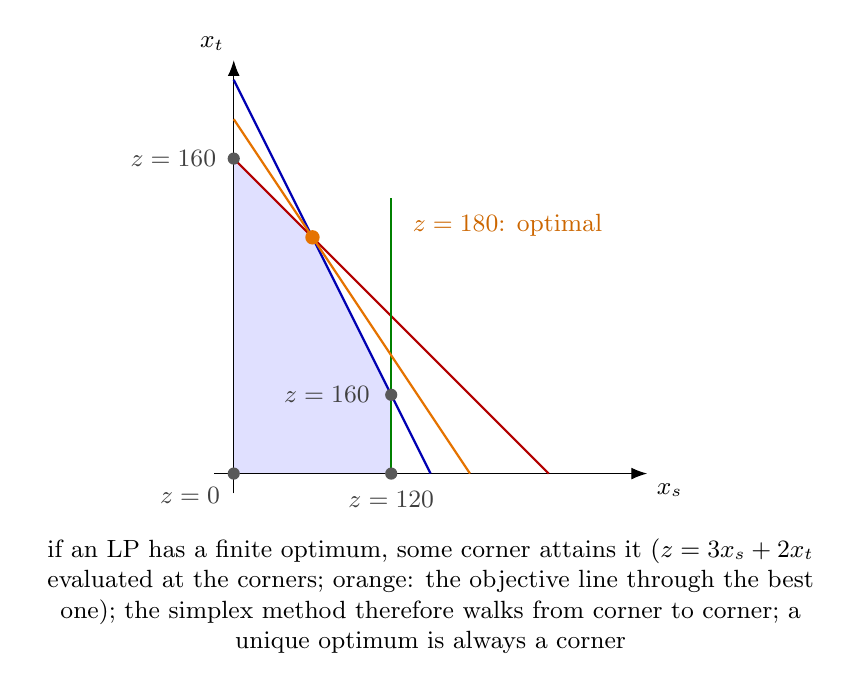
\begin{tikzpicture}[x=0.05cm, y=0.05cm, every node/.style={font=\small}, >={Latex[length=2mm]}]
	\fill[blue!12] (0,0) -- (40,0) -- (40,20) -- (20,60) -- (0,80) -- cycle;
	\draw[->] (-5,0) -- (105,0) node[below right] {$x_s$};
	\draw[->] (0,-5) -- (0,105) node[above left] {$x_t$};
	\draw[blue!70!black, thick] (50,0) -- (0,100);
	\draw[red!70!black, thick] (80,0) -- (0,80);
	\draw[green!50!black, thick] (40,0) -- (40,70);
	\draw[orange!90!black, thick] (60,0) -- (0,90);
	\foreach \p in {(0,0),(40,0),(40,20),(0,80)} {\fill[gray!70!black] \p circle (2.2pt);}
	\node[gray!50!black, font=\small, anchor=north east] at (-1,-1) {$z=0$};
	\node[gray!50!black, font=\small, anchor=north] at (40,-2) {$z=120$};
	\node[gray!50!black, font=\small, anchor=east] at (37,20) {$z=160$};
	\node[gray!50!black, font=\small, anchor=east] at (-2,80) {$z=160$};
	\fill[orange!90!black] (20,60) circle (2.6pt);
	\node[orange!80!black, font=\small, anchor=west] at (43,63) {$z=180$: optimal};
	\node[anchor=north, align=flush center, text width=10cm] at (50,-14) {if an LP has a finite optimum, some corner attains it ($z=3x_s+2x_t$ evaluated at the corners; orange: the objective line through the best one); the simplex method therefore walks from corner to corner; a unique optimum is always a corner};
\end{tikzpicture}
\end{document}
